\documentclass{article}

% if you need to pass options to natbib, use, e.g.:
% \PassOptionsToPackage{numbers, compress}{natbib}
% before loading nips_2016
%
% to avoid loading the natbib package, add option nonatbib:
% \usepackage[nonatbib]{nips_2016}

\usepackage[final]{nips_2016}

% to compile a camera-ready version, add the [final] option, e.g.:
% \usepackage[final]{nips_2016}

\usepackage[utf8]{inputenc} % allow utf-8 input
\usepackage[T1]{fontenc}    % use 8-bit T1 fonts
\usepackage{hyperref}       % hyperlinks
\usepackage{url}            % simple URL typesetting
\usepackage{booktabs}       % professional-quality tables
\usepackage{amsfonts}       % blackboard math symbols
\usepackage{nicefrac}       % compact symbols for 1/2, etc.
\usepackage{microtype}      % microtypography
\usepackage{fancyvrb,xcolor}
\usepackage{graphicx}


\title{Report for the Deep Learning Course Assignment 2 }

% The \author macro works with any number of authors. There are two
% commands used to separate the names and addresses of multiple
% authors: \And and \AND.
%
% Using \And between authors leaves it to LaTeX to determine where to
% break the lines. Using \AND forces a line break at that point. So,
% if LaTeX puts 3 of 4 authors names on the first line, and the last
% on the second line, try using \AND instead of \And before the third
% author name.

\author{
  Georgios Methenitis \\
  \texttt{georgios.methenitis@cwi.nl}
}

\begin{document}
% \nipsfinalcopy is no longer used

\maketitle

\begin{abstract}
In this assignment I got familiar with TensorFlow. I created a single hidden layer network with ReLU activation function to learn features for the CIFAR10 dataset.
The accuracy obtained in the test set, $0.46$, is similar to the neural network model of the previous assignment. 
\end{abstract}

\section{Task 1}
\begin{enumerate}
\item TensorFlow \emph{variables} are stored structures containing tensors, \emph{constants} are constant variables in Tensorflow, \emph{placeholders} are used in the place of variables at graph initialization when there are no variables. The differences are that constants cannot change their values in contrast with variables, and that placeholder are replacing variables at initialization phase.
\item There are two ways to declare variable in TensorFlow:
\begin{itemize}
\item \begin{small}
\begin{verbatim}
var = tf.get_variable("var_name", shape=[..., ...])
\end{verbatim}
\end{small}
\item \begin{small}
\begin{verbatim}
var = tf.Variable(tf.zeros([..., ...]), name="var_name")
\end{verbatim}
\end{small}
\end{itemize}

\item The command \texttt{tf.shape(x)} returns the shape of the input of tensor \texttt{x} in an 1-D vector, while \texttt{x.get\_shape()} return the size of the tensor.
\item
\item
\item A computational \emph{graph}, \emph{tensors} for the variables and \emph{operator}.
\item In variable scopes, variables can be created, adopting the prefix of the scope in their name, variable scopes enable variable sharing in different places in the code. The differences between name scopes and variable scopes is in the former creates an hierarchy for operations and variables in the graph, while the latter helps mostly in variable sharing.
\item You can freeze a variable tensor during training by setting \texttt{trainable=True} upon creating the variable, this way it will not get updated during optimization.
\item Yes Tensorflow uses automatic differentiation, while this can be a disadvantage for higher numbers of hidden layer due to dependencies.
The advantages are obvious, there is no need to compute difficult derivatives of high complexity.
\item One way is like the assignment, reading using a python script the data for every train step and feeding the data in the graph.
The other way is to read all the data from csv files at the beginning.
\end{enumerate}

\section{Task 2}
In this task I implemented the following functions in \texttt{mlp.py}, more specifically the \texttt{inference}, \texttt{loss}, and \texttt{accuracy}.

\begin{small}
\begin{verbatim}
  def inference(self, x):
    with tf.variable_scope('hidden', reuse=None):
      W = tf.get_variable("weights", shape=[x.get_shape()[1], self.n_hidden[0]],
       initializer=self.weight_initializer, regularizer=self.weight_regularizer)
      tf.histogram_summary("hidden_weights", W)
      b = tf.Variable(tf.zeros([self.n_hidden[0]]), name="bias")
      tf.histogram_summary("hidden_bias", b)

    with tf.variable_scope('output', reuse=None):
      w_out = tf.get_variable("weights", shape=[self.n_hidden[0], self.n_classes],
       initializer=self.weight_initializer, regularizer=self.weight_regularizer)
      tf.histogram_summary("output_weights", w_out)
      b_out = tf.Variable(tf.zeros([self.n_classes]), name="bias")
      tf.histogram_summary("output_bias", b_out)

    with tf.name_scope('relu_layer'):
      input = self.activation_fn(tf.matmul(x, W) + b)
    with tf.name_scope('linear_layer'):
      output = tf.matmul(input, w_out) + b_out

    return output
    
  def loss(self, logits, labels):

    loss = tf.reduce_mean(tf.nn.softmax_cross_entropy_with_logits(logits, labels, name=None))
    with tf.variable_scope("hidden", reuse=True):
      loss += 0.5 * tf.reduce_sum(tf.get_variable("weights")**2)
    with tf.variable_scope("output", reuse=True):
      loss += 0.5 * tf.reduce_sum(tf.get_variable("weights")**2)

    return loss
    
  def accuracy(self, logits, labels):
    correct_prediction = tf.equal(tf.argmax(labels, 1), tf.argmax(logits, 1))
    accuracy = tf.reduce_mean(tf.cast(correct_prediction, tf.float32))
    return accuracy
\end{verbatim}
\end{small}
I also implemented the function \texttt{train} in the file \texttt{train\_mlp.py}:
\begin{small}
\begin{verbatim}
def train():
  # placeholder for input and output tensors allowing to create operations and the computation graph
  x = tf.placeholder(tf.float32, shape=[None, 3072])
  y_ = tf.placeholder(tf.float32, shape=[None, 10])
  
  # model, namescopes for summary
  model = MLP()
  x_ = model.inference(x)
  with tf.name_scope('loss'):
    loss = model.loss(x_, y_)
  with tf.name_scope('accuracy'):
    accuracy = model.accuracy(x_, y_)
  with tf.name_scope('train_step'):
    train_step = tf.train.GradientDescentOptimizer(LEARNING_RATE_DEFAULT).minimize(loss)
  
  # session
  init = tf.initialize_all_variables()
  sess = tf.Session()
  sess.run(init)

  # merged summary for the graph, the loss and accuracy
  tf.scalar_summary('accuracy', accuracy)
  tf.scalar_summary('loss', loss)
  tf.histogram_summary("logits", x_) # logits histogram
  merged = tf.merge_all_summaries()


  train_writer = tf.train.SummaryWriter(LOG_DIR_DEFAULT + '/train', sess.graph)
  test_writer = tf.train.SummaryWriter(LOG_DIR_DEFAULT + '/test', sess.graph)

  for i in range(1, MAX_STEPS_DEFAULT+1):
      batch_xs, batch_ys = cifar10.train.next_batch(BATCH_SIZE_DEFAULT)
      __, Summary, l, acc = sess.run([train_step, merged, loss, accuracy],
      feed_dict={x: batch_xs, y_: batch_ys})
      train_writer.add_summary(Summary, i)

      if i % 100 == 0.0:
          batch_xs, batch_ys = cifar10.test.images, cifar10.test.labels
          __, Summary, l, acc = sess.run([train_step, merged, loss, accuracy],
           feed_dict={x: batch_xs, y_: batch_ys})
          test_writer.add_summary(Summary, i)

  train_writer.close()
\end{verbatim}
\end{small}

Figure~\ref{fig:acclosstrain} presents the accuracy and the loss in the training set recorded for every epoch.
The accuracy is higher than $0.45$ similar to the performance in the training set of the previous assignment, while the loss converges close to zero after 500 epochs.
\begin{figure}
\centering
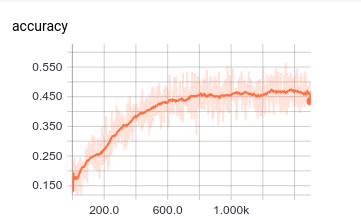
\includegraphics[width=0.5\textwidth]{loss.png}\	
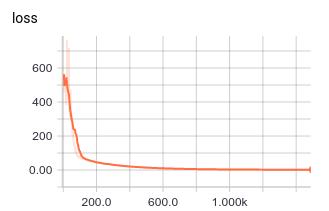
\includegraphics[width=0.45\textwidth]{accuracy.png}
\caption{Recorded accuracy and loss for the training set.}
\label{fig:acclosstrain}
\end{figure}
Figure~\ref{fig:acclosstest} presents the accuracy and the loss in the test set recorded every 100-epochs.
As you can see the accuracy drops after 1200 epochs, the model is overfitting.


\begin{figure}
\centering
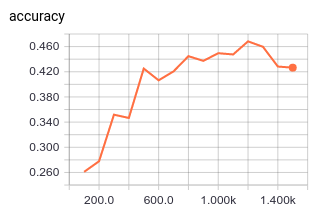
\includegraphics[width=0.5\textwidth]{accuracy_t.png}\	
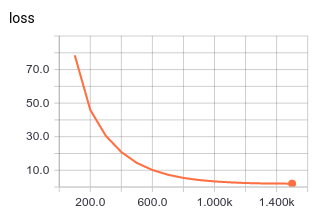
\includegraphics[width=0.45\textwidth]{loss_t.png}
\caption{Recorded accuracy and loss for the test set.}
\label{fig:acclosstest}
\end{figure}

Figure~\ref{fig:graph} presents the graph of the created model as this is illustrated by TensorBoard.
Using different namespaces where necessary we can illustrate the structure of the model.
You can see the two placeholder, one given as input to the relu layer and the second as the output of the linear layer, also connected to the accuracy module.
The two layer are connected to the loss module that then updates all weights in the output and hidden layers.



\begin{figure}
\centering
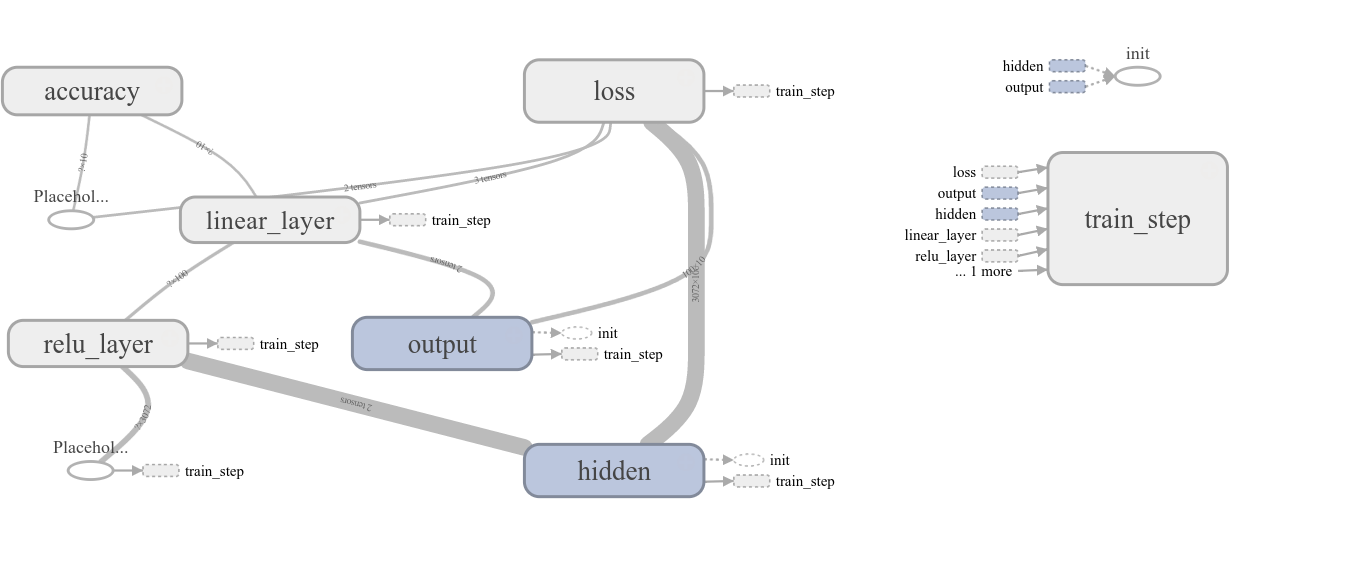
\includegraphics[width=0.9\textwidth]{graph.png}
\caption{Graph of the model.}
\label{fig:graph}
\end{figure}

Figure~\ref{fig:histogramsunits} presents the histograms of the weights and the biases in every unit of the model, in the hidden and the output units respectively.

\begin{figure}
\centering
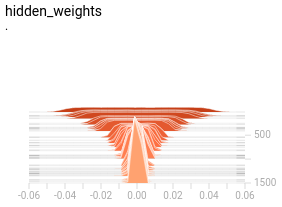
\includegraphics[width=0.3\textwidth]{hidden_weights.png}
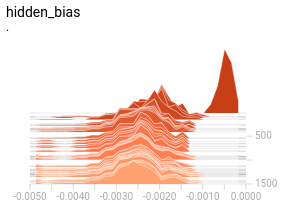
\includegraphics[width=0.3\textwidth]{hidden_bias.png}
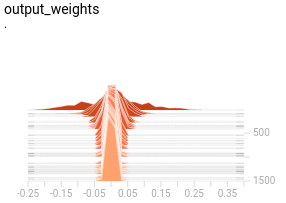
\includegraphics[width=0.3\textwidth]{output_weights.png}
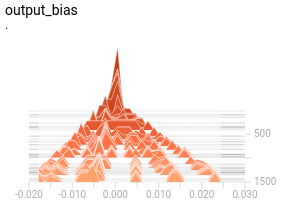
\includegraphics[width=0.3\textwidth]{output_bias.png}
\caption{Histograms of weights and bias in the hidden layer, and weights and bias in the output linear layer.}
\label{fig:histogramsunits}
\end{figure}

Figure~\ref{fig:histogramlogits} presents the histogram of the logits.
We can observe that only the variance of the logits change.

\begin{figure}
\centering
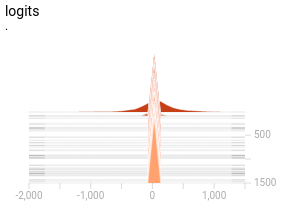
\includegraphics[width=0.4\textwidth]{logits.png}
\caption{Histograms of logits.}
\label{fig:histogramlogits}
\end{figure}


\section{Conclusion}
Although I did not have time to finish all the questions in the assignment I found it very useful.
Tensorflow provides an easy to use library to create and train models and visualize everything is happening during the training of the model.

\end{document}
